\input{../preamble}
\input{../usercommands}

\begin{document}
\vspace*{2cm}

{\centerline{\bf\huge AST2000 Lecture Notes}}

\vspace*{1cm}

\newcommand{\PartName}{2E}
\newcommand{\refproblem}[1]{\PartName.\ref{#1}}


{\centerline{\bf\LARGE Part \PartName}}\vspace*{0.25cm}
{\centerline{\bf\LARGE General Relativity: Gravitational lensing}}

\vspace*{1cm}

{\centerline{\underline{\LARGE Questions to ponder before the lecture}}}

\vspace*{1cm}

{\large
\begin{enumerate}
\item Newton's law of gravity shows the dependence of the gravitational force on a mass. In general relativity light is also affected by gravity, even though a photon is massless. Which property of the photon do you think decides the gravitational effect?
\item General relativity says that light is affected by a gravitational field, but would a ray of light also set up a gravitational field attracting nearby masses?
\item A solar eclipse in 1919 has become famous since the observation of stars close to the boundary of the eclipsed Sun was used to show the validity of the general theory of relativity. In which way do you think that the observation of these stars could be important for testing general relativity? And why during a solar eclipse?
\end{enumerate}

\begin{Figure}%[htb]
\centering
%\begin{center}
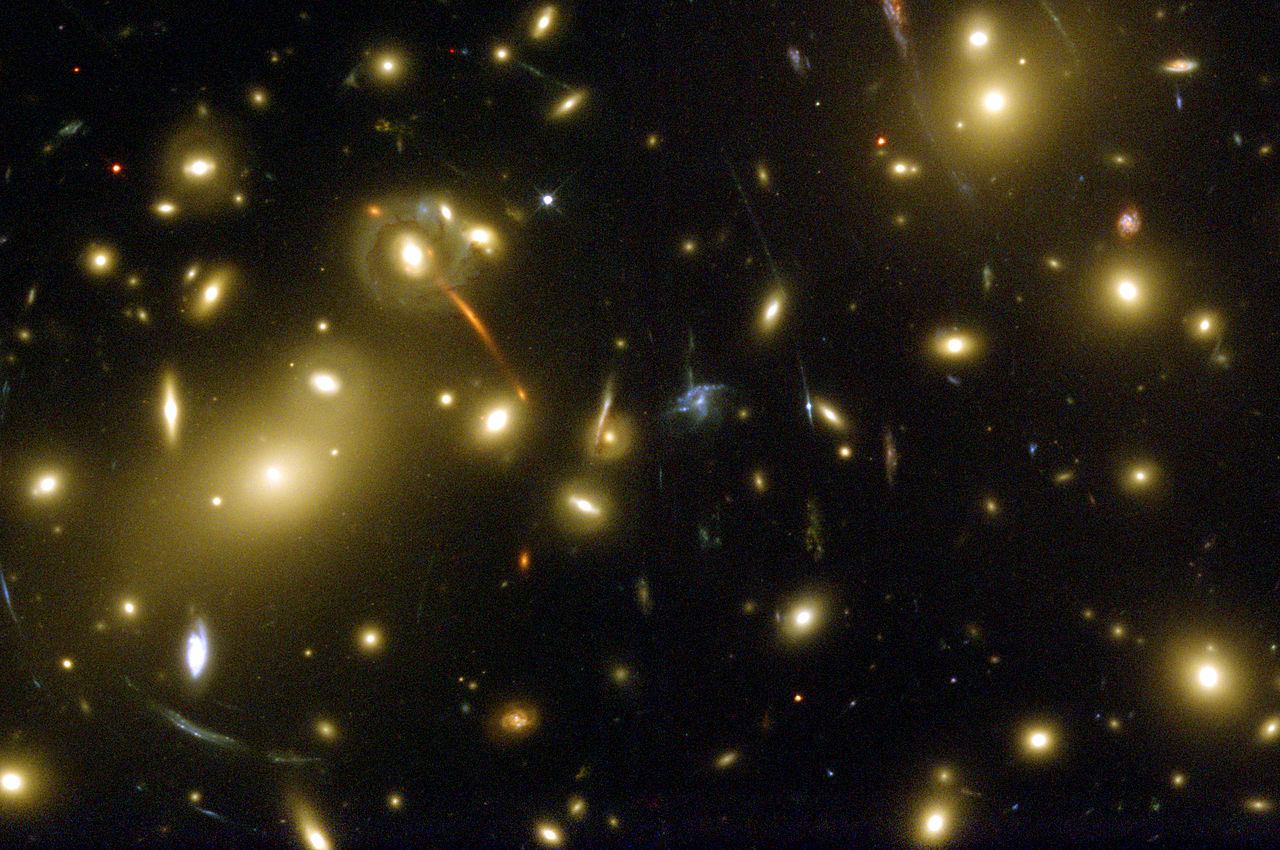
\includegraphics[width=0.9\textwidth]{lensing.jpg}
%\end{center}
\end{Figure}
%Image: strong lensing in Abell2218, credit: NASA/ESA


\clearpage
\vspace*{2cm}

{\centerline{\bf\huge AST2000 Lecture Notes}}

\vspace*{1cm}

{\centerline{\bf\LARGE Part \PartName}}\vspace*{0.25cm}
{\centerline{\bf\LARGE General Relativity:}}
{\centerline{\bf\LARGE Gravitational lensing}}


\vspace*{1cm}

\begin{multicols}{2}

\section{Motion of light in \ss spacetime}
\label{sect:motion}

There is one huge difference between Newton's and Einstein's theory of gravity. In the Einstein equation
\[
G_{\mu\nu}=8\pi T_{\mu\nu},
\]
energy (not only mass but total \emph{energy}) enters in the energy momentum tensor on the right hand side. This means that not only mass but also pure energy (for instance in the form of light or other kinds of radiation) give rise to curvature of spacetime as described by the left side of the equation. This means that light gives rise to a gravitational field. In the same manner, light is also affected by a gravitational field. We know that light follows a spacetime path such that $ds=0$. If the geometry of spacetime is the \ss geometry, this line will necessarily be different than if the geometry is Lorentz geometry. Hence the general theory of relativity predicts light rays to be deflected in a gravitational field. 

In this part we will mostly use expressions that we deduced in part 2D and apply these to light instead of matter. In a way, this part mostly involves practicing what you have already learned on examples involving light. For this reason, a large part of the calculations are found in the exercises while the main text will be used for interpreting the results.

We will now look at the step-by-step motion of a ray of light through \ss spacetime in the same way as we did for a rocket in the previous lecture. There is however one difference: We cannot use the proper time $\tau$ as the time parameter as $\Delta\tau=0$ always for light. We will instead use steps $dt$ measured on the far away clock.

In exercise \refproblem{prob:motion} you will show that the equations for step-by-step motion of light in \ss spacetime is given by
\begin{formbox}
\begin{align}
&\Delta r=\nonumber\\
&\pm \sst\sqrt{1-\sst\frac{(L/E)^2}{r^2}}\Delta t \label{eq:r}
\end{align}
\begin{equation}
\label{eq:phi}
r\Delta\phi=\pm\frac{L/E}{r}\sst\Delta t.
\end{equation}
\end{formbox}

These equations can again be used to describe the trajectory $(r,\phi)$ of light as the far-away time $t$ advances. 

We will use these equations to look at the speed of light in various cases. First we will emit a beam of light radially towards the center of the black hole. This is purely radial motion so $\Delta\phi=0$ and the angular momentum is zero $L=0$. Equation \ref{eq:r} then gives
\begin{equation}
\label{eq:vr}
v_r=\frac{dr}{dt}=-\sst.
\end{equation}
We see that the speed of light is not one as we are used to. Surprise, surprise! Special relativity was constructed based on the fact that the speed of light is one for all observers. In general relativity this is no longer true: We see here that the speed of light as measured in \ss coordinates $(r,t)$, the coordinates of the far-away observer, is different from one. And moreover as $r\rightarrow2M$ the speed of light goes to zero. Light slows down to zero close to the horizon (for the far-away observer), just as material particles do.

Now, this was measurements made by the far-away observer who makes measurements based on observations made by different local observers. What speed of light does a shell observer on a shell close to the horizon measure? Does he also see that light slows down and eventually stops? This was not the case for material particles, we will now make the same calculations for light.

The shell observer measures the speed of the light beam as it passes his shell. He makes the measurement in a short time interval such that he can be considered to be in a local inertial frame. Then his geometry is Lorentz geometry
\[
d\tau^2=dt_\sh^2-dr_\sh^2
\]
(you can show this last expression simply by inserting the expressions relating $dr$ and $dr_\sh$ as well as $dt$ and $dt_\sh$ into the \ss line element) and he will necessarily measure
\[
\frac{dr_\sh}{dt_\sh}=-1
\]
We can thus change the principle of invariant speed of light to: A \emph{local} observer, an observer who measures the speed of light directly, will always measure the speed of light to be one. The far-away observer who bases his measurement on the collection of observations from several different local observers will see a different speed of light.

In exercise \refproblem{prob:lightspeed} you will calculate the speed of a beam of light which moves tangentially.

\section{Impact parameter}
\label{sect:impact}

\begin{Figure}
\centering
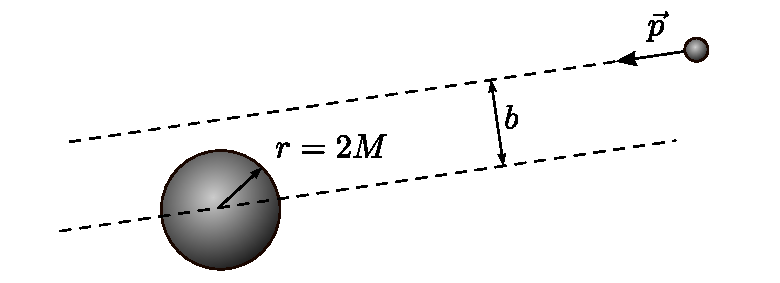
\includegraphics[width=\textwidth]{fig_18-1.pdf}
\captionof{figure}{Defining the impact parameter.\label{fig:b}}
\end{Figure}


To study the motion of light in a gravitational field we need to define the {\it impact parameter} $b$. The impact parameter is used in many fields of physics and astrophysics, for instance to study colliding particles. In figure \ref{fig:b} we see a large central mass $M$ (for instance a black hole) and a small particle far away from the central mass moving in any given direction. Draw a line passing through the particle going in the direction of motion of the particle. Then draw another line which is parallel to the first line but which passes through the center of the black hole. The distance between these two lines is called the impact parameter. It is important to note that the first line is drawn on the basis of the movement of the particle when the particle is so far away that it has not yet been influenced by the gravitational field. We will soon see that this impact parameter will decide the future motion of the photon.


\begin{Figure}
\centering
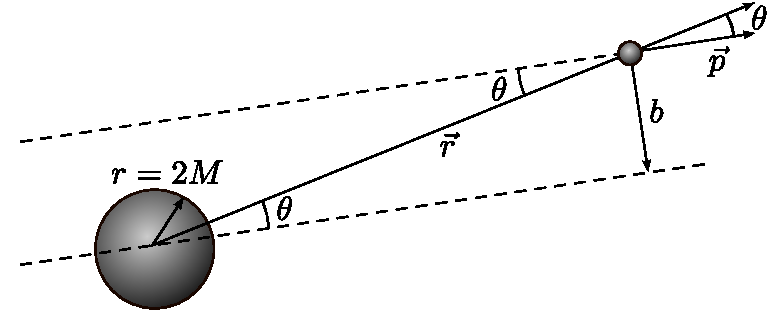
\includegraphics[width=\textwidth]{fig_18-2.pdf}
\captionof{figure}{The impact parameter expressed in terms of angular momentum.\label{fig:b2}}
\end{Figure}


We can calculate the angular momentum of the photon when it is still far away as
\[
L=|\vec{r}\times\vec{p}|=rp\sin{\theta}=pb.
\]
The angle $\theta$ is the angle between $\vec{r}$ pointing at the particle from the center of the black hole and $\vec{p}$ the momentum vector of the particle. The geometry is shown in figure \ref{fig:b2} explaining why we can write $b=r\sin{\theta}$. Thus, the impact parameter of a particle can be written as the ratio between angular and linear momentum
\begin{formbox}
\[
b=\frac{L}{p}.
\]
\end{formbox}
For a photon, we have that $p=E$ so that
\[
b=\frac{L}{E}.
\]
(valid for photons only). Using this, we can rewrite equation (\ref{eq:r}) and (\ref{eq:phi}) using the impact parameter as (check!)
\begin{align}
\label{eq:r2}
\frac{dr}{dt}&=\pm\sst\sqrt{1-\sst\frac{b^2}{r^2}}\\
\frac{rd\phi}{dt}&=\pm\frac{b}{r}\sst.
\end{align}
In the exercises you will show that the equations of motion for a photon can be written as 
\[
A=Bv_\mathrm{r,shell}^2+V_\mathrm{eff}(r)^2,
\]
where $A=B=1/b^2$ and 
\begin{formbox}
\[
V_\mathrm{eff}(r)=\frac{1}{r}\sqrt{\sst}.
\]
\end{formbox}
We see again that we have an equation on the same form as equation (4) in the previous lecture. We know that we need to compare the value of the constant A (which usually contains the energy $E/m$, but which this time contains only the impact parameter) with the shape of the effective potential. For a material body we showed in the previous lecture that it was the energy $E/m$ which appeared in the constant $A$ and therefore it was the value of this energy which decided whether the particle would move in an orbit, escape to infinity or be swallowed by the black hole. For the photon, we see that it is the impact parameter alone and not the energy which decides its destiny.


\begin{Figure}
\centering
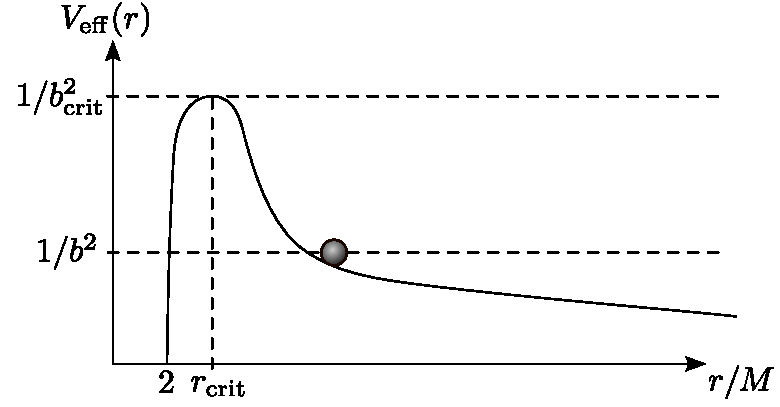
\includegraphics[width=\textwidth]{fig_18-3.pdf}
\captionof{figure}{The effective potential for light.\label{fig:pot}}
\end{Figure}


In figure \ref{fig:pot} we see the effective potential for light. The first thing which strikes us in this figure is that the potential does not exhibit a minimum as all the other potentials we have discussed so far. The consequence is that light cannot go in a stable orbit. If $1/b^2$ is lower than the peak in the figure, the light will approach the black hole, be deflected in some direction and escape to infinity (do you see why?). If $1/b^2$ is larger than the value at the peak in the figure, light will be captured by the black hole. In the exercises you will show that the peak in the potential is located at $r=3M$ for which $1/b^2=1/(27M^2)$. 

Light which approaches the black hole with $1/b^2$ equal to the value of the potential at the peak $1/(27M^2)$ will go in an unstable orbit at $r=3M$. For this reason $r=3M$ is called the {\it light sphere}. All the stars around a black hole radiate light in all possible directions with a huge range of impact parameters. There will always be light approaching the black hole with an impact parameter equal to the critical impact parameter $1/b_\mathrm{crit}^2=1/(27M^2)$ such that the light will orbit the black hole at the light sphere. A shell observer at the light sphere will see a ring around the black hole with several copies of images of the stars in the sky. The light will not stay in the light sphere for very long: Staying at the peak of the potential means being in an unstable orbit. Tiny fluctuations in the impact parameter will make the light either plunge into the black hole or escape. Coincidences will decide. This is exactly what we saw for material bodies approaching the black hole with an energy such that it balanced on the peak of the potential for a few revolutions and then either plunged or escaped.

\pagebreak[1]

\section{Deflection of light}
\label{sect:deflection}

In figure \ref{fig:gravlens1} we see light approaching a star at a large distance with an impact parameter such that the light will pass the star, be deflected and then escape to infinity. The question is with how large an angle $\Delta\phi$ the light is deflected. If the light is significantly deflected by a star it would mean that we cannot trust the position of objects that we observe on the sky: If the light from distant galaxies is deflected by all the stars it passes on the way to Earth, the original direction of the light and hence of the galaxy would be lost. We need to calculate how large the deflection is to find out whether this could be a problem for astronomical observations or not.


\begin{Figure}
\centering
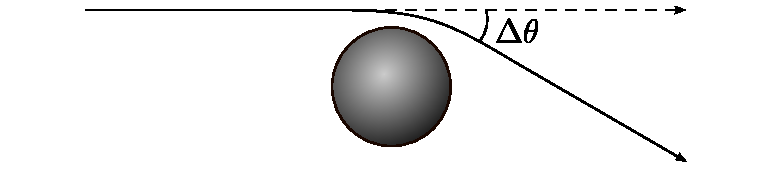
\includegraphics[width=\textwidth]{fig_18-4.pdf}
\captionof{figure}{Deflection of light by a star. The dotted line is the direction light would have taken if no deflection had taken place.\label{fig:gravlens1}}
\end{Figure}

\begin{Figure}
\centering
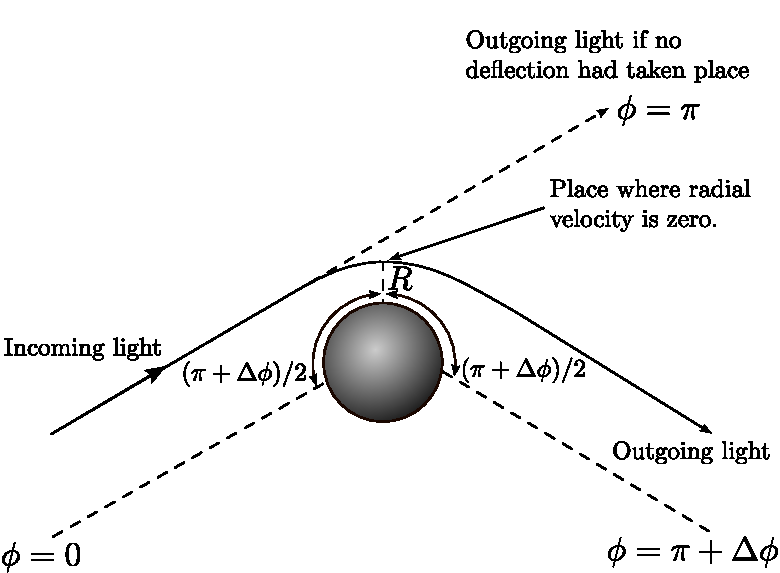
\includegraphics[width=\textwidth]{fig_18-5.pdf}
\captionof{figure}{Deflection of light by a star. Symmetry makes the situation equal on either side of the point where the distance between the light beam and the star is minimal $r=R$ and the radial velocity of the beam is zero.\label{fig:gravlens2}}
\end{Figure}


In figure \ref{fig:gravlens2} we show the situation in detail: Light with impact parameter $b$ is approaching a star of mass $M$. We have defined the $\phi$ coordinate such that $\phi=0$ when the light is infinitely far away. If light had not been deflected by the gravitational field, it would continue in a straight line to infinity at $\phi=\pi$. But we know that the light is deflected an angle $\Delta\phi$ such that the light goes to infinity at $\phi=\pi+\Delta\phi$. We will now study light which has an impact parameter $b$ such that it passes the star with radial shell velocity $v_\mathrm{r,shell}$ equal to zero at a distance $R$ from the star (see figure \ref{fig:gravlens2}). In order to calculate the deflection $\Delta\phi$ for this beam of light we will use the equations of motion for light in \ss geometry given by equations (\ref{eq:r}) and (\ref{eq:phi}). Dividing the two equations by each other we find
\[
d\phi=\frac{dr}{r^2\sqrt{\frac{1}{b^2}-\frac{1}{r^2}\sst}}.
\]
We need to integrate this equation to obtain the deflection $\Delta\phi$ from the particle arrives at $r=\infty,\phi=0$ to $r=\infty,\phi=\pi+\Delta\phi$. Because of symmetry, it is sufficient to find the deflection $\Delta\phi/2$ occurring during the trip from $(r=\infty,\phi=0)$ to $(r=R,\phi=\pi/2+\Delta\phi/2)$ (see again figure \ref{fig:gravlens2}). The symmetry of the problem tells us that this deflection equals the deflection occurring during the trip from $(r=R,\phi=\pi/2+\Delta\phi/2)$ to $(r=\infty,\phi=\pi+\Delta\phi)$. The geometry of the problem is detailed in figure \ref{fig:gravlens2}. We therefore need to perform the following integration (integrating the previous equation)
\begin{equation}
\label{eq:defintegral}
\int_0^{\pi/2+\Delta\phi/2}d\phi=\int_{\infty}^R\frac{dr}{r^2\sqrt{\frac{1}{b^2}-\frac{1}{r^2}\left(1-\frac{2M}{r}\right)}}.
\end{equation}
You will perform this integral in exercise \refproblem{prob:deflection}. Note that solving this integral is not just a test of mathematical knowledge, it also needs a thorough understanding of the general relativity we have learned so far. The result you will show is
\begin{formbox}
\begin{equation}
\label{eq:deflection}
\Delta\phi=\frac{4M}{R}.
\end{equation}
\end{formbox}


\begin{figure*}
\fcolorbox{black}{yellow}{\parbox{\dimexpr \linewidth-2\fboxsep-2\fboxrule}{
\begin{minipage}{0.6\textwidth}%{\dimexpr\linewidth-2\fboxsep-2\fboxrule}\parskip=6pt
{\small
\fontfamily{bch}\selectfont
\vspace*{-0.2cm}\hspace*{-0.15cm}\fcolorbox{black}{black}{\bf\color{white} Fact sheet:\color{black}} 
This illustration shows how gravitational lensing works. The gravity of a large galaxy cluster is so strong that it bends, brightens and distorts the light of a distant galaxy behind it. In this case observers on Earth see two images of the same object. Note that in reality, the distant galaxy is much farther away than it appears here. Gravitational lensing is an impressive astronomical tool; it can be used to detect exoplanets, learn about distant galaxies and galaxy clusters, and measure dark matter, dark energy and the age of the universe. Astronomer Fritz Zwicky postulated in 1937 that gravitational light bending could allow galaxy clusters to act as gravitational lenses. It was not until 1979 that this exotic phenomenon was confirmed observationally with the discovery of the "Double Quasar" QSO 0957+561. The Norwegian astronomer Sjur Refsdal made pioneering work on gravitational lensing and microlensing in the 1960s, 70s and 80s. (Figure: NASA, ESA \& L. Calcada)
}
\end{minipage}%\hspace*{0.5cm}
\ \ \ \ \ \ \begin{minipage}{0.35\textwidth}
\centering
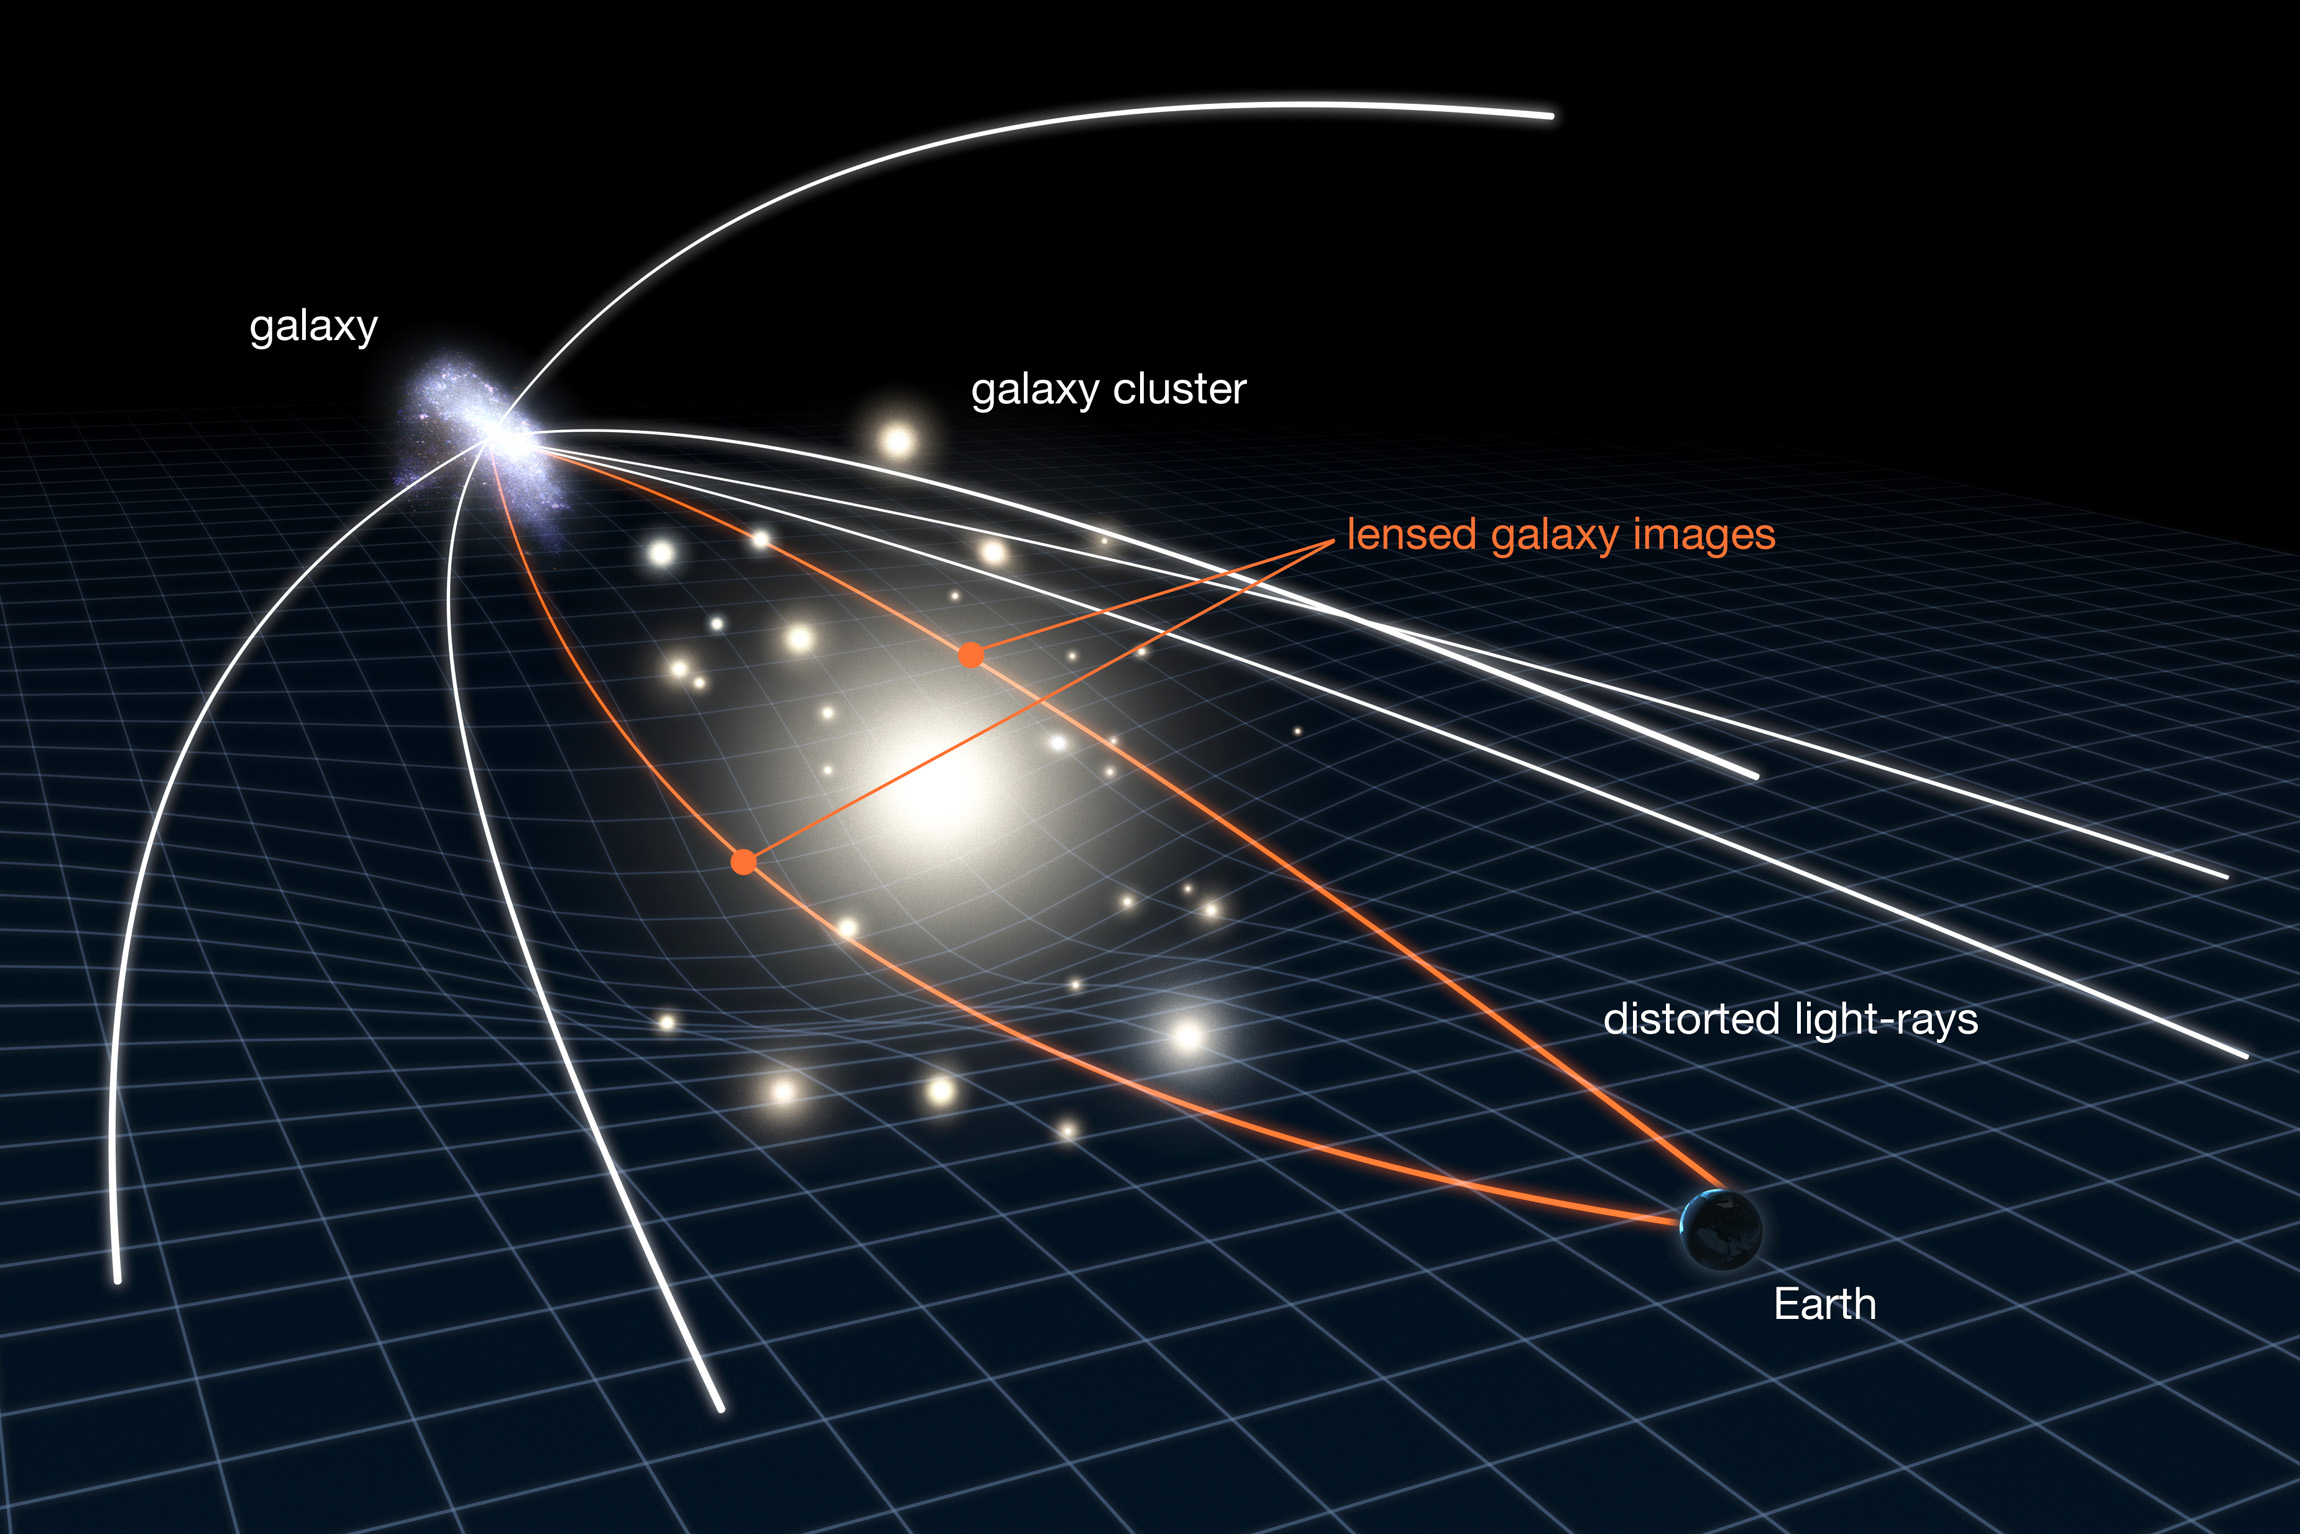
\includegraphics[width=\textwidth]{GL_cluster_NASA.jpg}
%\end{wrapfigure}
%\end{center}
%\end{figure*}
\end{minipage}
}}
\end{figure*}


In exercise \refproblem{prob:eclipse}  you will see how close to a star light needs to pass for the deflection to be important. You will also show that light from stars which pass close to the surface of the Sun will be deflected significantly. Stars which we observe in a direction close to the surface of the Sun will thus be observed in the wrong position on the sky. The stars will be shifted due to the deflection of light. This is a good test of the theory of general relativity: We now have a formula to predict exactly by how large angle the position of a star on the sky will change when viewed close to the surface of the Sun. The problem is that the light from the Sun is so strong that we cannot see stars which have a position on the sky close to the Sun. The only possibility to observe these stars is during a total solar eclipse. During a solar eclipse in 1919, this effect was measured for the first time: Stars which were seen close to the surface of the Sun were measured to have shifted their position with exactly the angle predicted by general relativity. This was the discovery which made Einstein famous.

\section{Gravitational lensing}
\label{sect:lensing}

\begin{Figure}
\centering
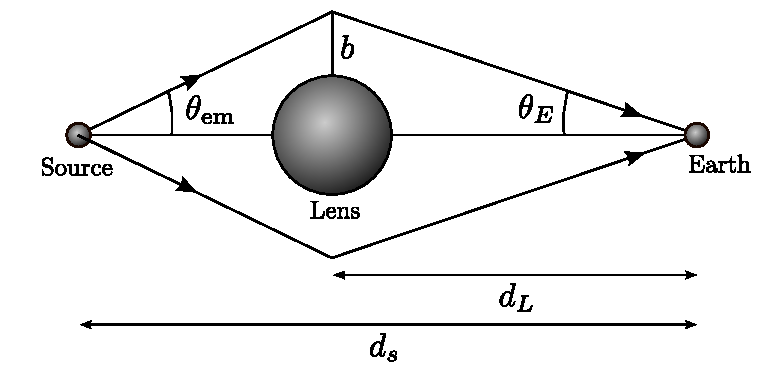
\includegraphics[width=\textwidth]{fig_18-6.pdf}
\captionof{figure}{The source on the left (a quasar), the lens in the middle (a cluster of galaxies) and the Earth on the right receiving the radiation from the quasar from several angles.\label{fig:gravlens3}}
\end{Figure}


The gravitational deflection of light is used today to study the most remote objects in the visible universe. In figure \ref{fig:gravlens3} we show a typical situation. A quasar (a black hole with gas falling into it producing strong radiation at several wavelengths, quasars are one of the most powerful radiation sources in the universe) is located at a distance $d_S$ and a cluster of galaxies with mass $M$ is located at distance $d_L$. The indices $S$ and $L$ refer to 'source' and 'lens'. The quasar is the source of light and the cluster of galaxies deflects this light similar to an optical lens. For this reason we call the cluster of galaxies for the 'lens' and the effect of light deflection is called {\it gravitational lensing}. It's important to note that although figure \ref{fig:gravlens3} is a good illustration it's physically incorrect. Gravitational lensing will not happen abruptly but smoothly, this error will be handled in exercise \refproblem{prob:lensing_figure}.

The limiting angle $\theta_\mathrm{em}$ (see figure \ref{fig:gravlens3}) is the angle that the light emitted from the quasar needs to have in order to reach Earth. Light emitted with a smaller angle will be deflected too much, light emitted with a larger angle will be deflected too little. Only light with angle $\theta_\mathrm{em}$ will be deflected in such a way that the light will reach us and we will see the quasar. The figure shows only a two dimensional plane, taking into account the three dimensional geometry of the problem, light emitted with an angle $\theta_\mathrm{em}$ will reach us from all direction the result being that we see the quasar as a ring of light around the cluster (see figure \ref{fig:ring}). We call this ring an {\it Einstein ring}. The angle $\theta_E$ is the observed angular radius of the Einstein ring (you find the angle both in figure \ref{fig:gravlens3} and \ref{fig:ring} check that you understand the relation between the two figures). In the exercises, you will show that this angle can be written as
\begin{formbox}
\begin{equation}
\label{eq:lensing}
\theta_E=\sqrt{\frac{4M(d_S-d_L)}{d_Ld_S}},
\end{equation}
\end{formbox}
which is called the {\it lensing formula}.

\begin{Figure}
\centering
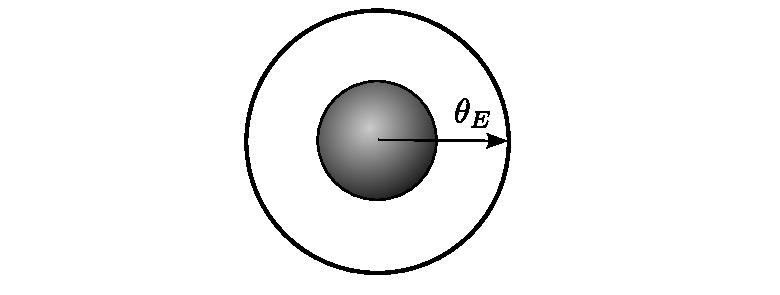
\includegraphics[width=\textwidth]{fig_18-7.pdf}
\captionof{figure}{The cluster of galaxies in the middle and the Einstein ring being the lensed image of the quasar behind. The angular radius of the ring is $\theta_E$.\label{fig:ring}}
\end{Figure}

\begin{Figure}
\centering
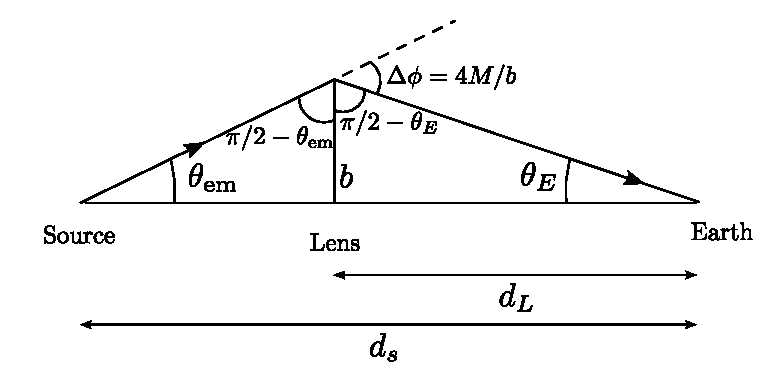
\includegraphics[width=\textwidth]{fig_18-8.pdf}
\captionof{figure}{Detailed geometry of the situation in figure \ref{fig:gravlens3}.\label{fig:gravlens4}}
\end{Figure}

From spectroscopic measurements, the distances $d_S$ and $d_L$ of the quasar and the cluster are normally known. The angular radius of the Einstein ring can be measured by observations. Combining these numbers, the lensing formula can be used to find the mass of a cluster of galaxies. We remember from previous lectures that we can use the virial theorem to find the mass of clusters of galaxies. The mass estimates of clusters obtained using the lensing formula is based on assumptions very different from those used in the virial theorem approach. Thus we have two independent measurements of the mass of the cluster. These two ways of measuring mass are in good agreement taking into account the uncertainties in the two methods. Both methods tell us that there is far more dark than luminous matter in clusters of galaxies being another confirmation of the existence of dark matter.
\begin{figure*}
\fcolorbox{black}{yellow}{\parbox{\dimexpr \linewidth-2\fboxsep-2\fboxrule}{
\begin{minipage}{0.6\textwidth}%{\dimexpr\linewidth-2\fboxsep-2\fboxrule}\parskip=6pt
{\small
\fontfamily{bch}\selectfont
\vspace*{-2.1cm}\hspace*{-0.15cm}\fcolorbox{black}{black}{\bf\color{white} Fact sheet:\color{black}} 
Believe it or not, this is a real picture of the sky, taken with the Hubble Space Telescope. The gravity of an unusually massive galaxy (the fuzzy yellow object in the middle) has gravitationally distorted the light from a much more distant blue galaxy. More typically, such light bending results in two discernible images of the distant galaxy, but here the lens alignment is so precise that the background galaxy is distorted into nearly a complete Einstein ring! The blue galaxy's redshift is approximately 2.4. This means we see it as it was only about 3 billion years after the Big Bang.(Figure: ESA/Hubble \& NASA)
}
\end{minipage}%\hspace*{0.5cm}
\ \ \ \ \ \ \begin{minipage}{0.35\textwidth}
\centering
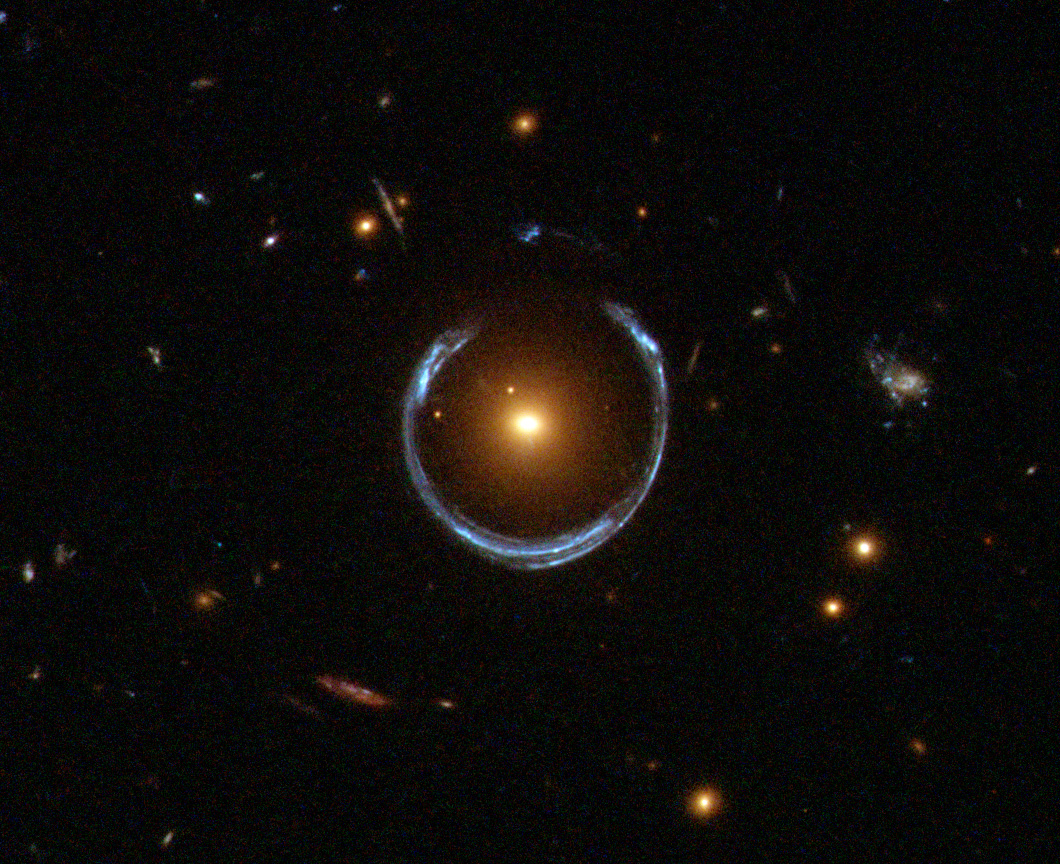
\includegraphics[width=\textwidth]{GL_ring_HST.jpg}
%\end{wrapfigure}
%\end{center}
%\end{figure*}
\end{minipage}
}}
\end{figure*}
To obtain an Einstein ring, the quasar needs to be exactly behind the center of the cluster of galaxy. Furthermore the cluster needs to have a spherical mass distribution. This is basically never the case, a complete Einstein ring is very rarely observed. What we rather see are small arcs around the cluster. By studying these arcs combined with more advanced theory of gravitational lensing, one can even infer the distribution of mass in the cluster of galaxies.

Finally I will mention another important use of gravitational lensing based on {\it microlensing}. The idea of microlensing is based on the following observation: The lens deflects light from the source towards Earth, light which otherwise would not have reached us. The lensing effect increases the total amount of photons from the quasar arriving to the Earth. Gravitational lensing does not only happen at the scale of clusters of galaxies. Even if an object passes in front of a star, gravitational lensing occurs. In this case, the Einstein ring is so small that it cannot be resolved on the sky. Only one effect of the lensing is directly observable: The fact that more light is directed towards us. The flux we receive from the star increases when the object is in front of the star. This is called microlensing. 

Microlensing has been used to look for 'lumps' of dark matter in the Milky Way, so-called MAssive Compact Halo Objects (MACHO). If these MACHOs, lumps of dark matter orbiting the center of the Milky way, exist they should cause microlensing of stars in the LMC and SMC (Large and Small Magellanic Clouds). The LMC and SMC are dwarf galaxies orbiting the center of the Milky Way. The MACHOs are expected to have orbits between us and the Magellanic clouds. When the MACHOs pass in front of stars in the Magellanic clouds microlensing will increase the flux from these stars for a few days or weeks. An extensive search program is running looking for these microlensing events in the Magellanic clouds in order to get closer to the solution of the dark matter mystery.

\newpage


%\TileWallPaper{51.5pt}{11.5pt}{noisy_grid.png}
\pagestyle{headings}
\section{Exercises}
\newcounter{problem}
\newcommand{\newproblem}[1]{\refstepcounter{problem}\label{#1}{\bf Exercise \refproblem{#1}}}

\newproblem{prob:motion}

Relevant theory: Section \ref{sect:motion}.\newline
The goal of this exercise is to show equations \ref{eq:r} and \ref{eq:phi} for the step-by-step motion of a ray of light.\newline You get three hints:
\begin{enumerate}
\item You can start from equations (2) and (3) in part 2D.
\item You can use the general relativistic expression for energy to substitute $d\tau$ with $dt$.
\item When you have obtained expressions with $dt$ instead of $d\tau$, there is one last question: what is the mass of a photon?
\end{enumerate}
Now check that you arrived exactly at equations \ref{eq:r} and \ref{eq:phi}.

\vspace{0.5cm}


\newproblem{prob:lightspeed_radial}

This exercise continues where exercise 2C.5 ended. Please go back and repeat what you did in exercise 2C.5, in particular you should look at the videos of both frames in 2C.5 and make sure you understand what happens. It is important that you read through the questions in exercise 2C.5 before you continue.

You will now need the xml-files for this exercise. These videos are the same as the videos for 2C.5, with one important difference: now the light travel time has been included. In the 2C.5 videos, you assumed the light to travel at infinite speed such that you saw the light signals immediately as they were emitted. Now you see the light signal when it actually reaches you, this is what you would really see. Please do not watch the videos for this exercise yet.

\begin{enumerate}
\item Look at the frame one video (observing the space craft from the shell) of 2C.5, do not look at the video for this exercise yet. Use equation \ref{eq:vr} to judge what you {\bf think} will change (no calculations, just considerations) in the new video and how.
\item Plot the time differences between the lights signal against the earlier number of total time intervals. Explain the trend, why does this trend occur? When creating the xml-files use the argument \texttt{write\_text=True} to generate a text file with this information. To make your life even easier use the numpy function \texttt{x,y = loadtxt('name\_of\_txt\_file.txt')} to load the information into arrays, where x is the interval number and y is the corresponding time difference.
\item Now watch both videos, the one with and without light travel included for frame one. Were there any notable differences?
\item  Watch the video corresponding to frame two without light travel included, do not look at the video that includes light travel.  Show that the distance $\Delta r_\gamma$ that a photon approaching the space craft travels during a time interval $\Delta\tau$ on the space craft clock is given by
\[
\Delta r_\gamma=-\frac{1-\frac{2M}{r_\gamma}}{1-\frac{2M}{r}}\frac{E}{m}\Delta\tau
\]
where $r_\gamma$ is the position of the photon and $r$ is the position of the space craft. Use this equation to judge  what you {\bf think} will change (no calculations, just considerations) in the new video and how.
\item Watch the video corresponding to frame 2, with both light travel included and not included. Thereafter plot the time intervals just as done in exercise 2. Did you expect this? Can you explain this?
\end{enumerate}



\newproblem{prob:lightspeed}

Relevant theory: Section \ref{sect:motion}.\newline
In this exercise you will show that the speed of a light beam (measured from the far-away obsever) which moves tangentially ($\Delta r=0$) is given by
\[
v_\phi=\sqrt{\sst}.
\]

In the following you will need equations \ref{eq:r} and \ref{eq:phi}:
\begin{enumerate}
\item Write the equation for tangential speed $v_\phi$ expressed by the distance $r$, a tiny movement $d\phi$ and a tiny time step $dt$.
\item Find an expression for $\frac{L}{E}$ for an object which moves tangentially (with no radial speed component)
\item Combine these two results and prove the equation above for $v_\phi$.
\item Does light move faster when it moves radially or tangetially? (measured from the far-away obsever)
\item From the equations of radial and tangential velocity you can clearly see that the light beams can have a velocity less than the speed of light. But what would a shell observer measure in his initial system? \textbf{Hint:} No calculations needed.

\end{enumerate}

\vspace{0.5cm}



\newproblem{prob:lightpot}

Relevant theory: Section \ref{sect:impact}.\newline
Use the equations of motion for a photon (equation \ref{eq:r2}) to show that the radial light speed $dr_\sh/dt_\sh$ observed by the shell observer can be written as
\begin{equation}
\label{eq:vrshell}
\frac{1}{b^2}\left(\frac{dr_\sh}{dt_\sh}\right)^2=\frac{1}{b^2}-\frac{\sst}{r^2}.
\end{equation}
Look at equation (7) and (8) from part 2D and show that we can define an effective potential for light (based on the shell velocity rather than the velocity $dr/dt$) as
\[
V(r)=\sqrt{\frac{\sst}{r^2}}.
\]

\vspace{0.5cm}

\newproblem{prob:bcrit}

Relevant theory: Section \ref{sect:impact}.
\begin{enumerate}
\item By taking the derivatives of the effective potential for light, show that the potential has only one extremal point which is a maximum. Explain why this means that there are no stable orbits for light. 
\item Show that this maximum occurs at $r=3M$ and explain why we call this radius the light sphere. 
\item Show that the criterion deciding whether light will escape a black hole or plunge into it is given by the critical impact parameter as
\[
b_\mathrm{crit}=3\sqrt{3}M\approx5.2M
\]
\end{enumerate}

\vspace{0.5cm}


\newproblem{prob:deflection}

Relevant theory: Section \ref{sect:deflection}.\newline
Here we will solve the integral in equation \ref{eq:defintegral} to obtain equation \ref{eq:deflection} for the deflection of a light beam from a gravitational field.
\begin{enumerate}

\item To make the integration easier we will make the substitution $u=R/r$. Show that you get:
\[
\int_0^{\pi/2+\Delta\phi/2}d\phi=\frac{1}{R}\int_0^1\frac{du}{\sqrt{\frac{1}{b^2}-\frac{u^2}{R^2}\left(1-\frac{2M}{R}u\right)}}.
\]
\item Before integrating there is one more information which we have not used: The fact that we know the impact parameter $b$. What is the radial shell velocity at $r=R$? 
\item In problem \refproblem{prob:lightpot} you found an expression for the radial shell velocity of light (equation \ref{eq:vrshell}) as a function of distance and impact parameter. Setting the radial velocity to the value you found in the previous question should give you:
\begin{equation}
\label{eq:vrshell2}
\frac{1}{b^2}=\frac{1}{R^2}\left(1-\frac{2M}{R}\right),
\end{equation}
\item Use this result to show that
\[
\frac{\pi}{2}+\frac{\Delta\phi}{2}=\int_0^1\frac{du}{\sqrt{\left(1-\frac{2M}{R}\right)-u^2\left(1-\frac{2M}{R}u\right)}}.
\]
\item Argue why $R\gg2M$ for a star (check that this must be so for the Sun: find the radius of the Sun expressed in Solar masses. Also argue why $R$ must be larger than the radius of the star.
\item We now define $x=M/R$. You just argued why $x\ll1$ and we can therefore try to Taylor expand the integrand in the small value $x$. Show that the integrand now can be written as
\[
f(x)=(1-2x-u^2(1-2xu))^{-1/2}\approx f(0)+f'(0)x
\]
\item Show that we get
\begin{align*}
&\frac{\pi}{2}+\frac{\Delta\phi}{2}\\
%&=\underbrace{\int_1^0\frac{du}{\sqrt{1-u^2}}}_{\pi/2}+\\
&=\int_1^0\frac{du}{\sqrt{1-u^2}}+\\
%&+\frac{M}{R}\underbrace{\int_1^0\left[\frac{1}{(1-u^2)^{3/2}}-\frac{u^3}{(1-u^2)^{3/2}}\right]du}_2.
&+\frac{M}{R}\int_1^0\left[\frac{1}{(1-u^2)^{3/2}}-\frac{u^3}{(1-u^2)^{3/2}}\right]du.
\end{align*}
\item Look up the solution to these integrals in tables (or use \url{http://www.wolframalpha.com/calculators/integral-calculator/})
\item Show that we get
\[
\frac{\Delta\phi}{2}=\frac{2M}{R},
\]
and thereby the expression in equation \ref{eq:deflection}.
\end{enumerate}

\vspace{0.5cm}

\newproblem{prob:eclipse}

Relevant theory: Section \ref{sect:deflection}.\newline
In 1919 a solar eclipse gave one of the first opportunities to check the validity of Einstein's theory. Stars which appear very close to the Sun can normally not be seen due to the much stronger light from the Sun. Only light from the stars which appear very close to the Sun on the sky would be significantly affected by the gravitational field of the Sun. The only possibility we have to see these stars is during a solar eclipse. The light from the Sun is blocked and the stars can be seen. If the light from these stars pass close to the surface of the Sun they will be deflected by the solar gravitational field. This deflection will shift the position of the star on the sky.
\begin{enumerate}
\item Make a drawing of the earth, the sun and a small illuminated object all aligned. The distance between the sun and earth is equal to that of the sun and the object. Draw how the light from the objects gets shifted from the sun onto the earth. From the earth, where is the apparent position of the illuminated object? Is the apparent position of the object shifted towards or away from the central line? 

\item Draw on the necessary angles on the drawing to show that the shift in apparent angular position is $\alpha=\Delta \phi$.
\end{enumerate}
In reality, light won't nearly be shifted as much as in the drawing, let's now calculate the total shift they should have measured in 1919.
\begin{enumerate}
\setcounter{enumi}{2}
\item Calculate the angular shift in position in arc seconds assuming that light passes very close to the solar surface.
\item Repeat the previous calculation for the Moon. Is the same effect measurable for stars close to the Moon? (Here you need the mass of the Moon)
\end{enumerate}

\vspace{1cm}

\newproblem{prob:lensing_figure}

Relevant theory: Section \ref{sect:deflection} and \ref{sect:lensing}.\newline
In the first paragraph of section \ref{sect:lensing} it was stated that figure \ref{fig:gravlens3} is physically incorrect. In this exercise you will delve into why the figure is incorrect and make the necessary adjustments to correct it.
\begin{enumerate}
\item Use symmetry arguments around the line 'b' to determine the correct trajectory around said line. \textbf{Hint:} Shouldn't the triangles be equal when mirroring around an axis? 
\item Run the program that calculates the trajectory of light around a black hole. The program plots two plots both with three lines: the actual trajectory, a triangular illustration and the symmetry line. The first plot corresponds to the actual trajectory and the second is the trajectory but the coordinates is shifted so the symmetry line aligns with the x-axis. You might have to zoom rather close to see the symmetry, but not to close, remember numerical error. From which points does the symmetry vector start and end?
\end{enumerate}
From physical measurements we know that light from far away sources get lensed around large objects onto us. This still applies even thought the length between the light source and lens and between the lens and earth is different, but for all cases symmetry is conserved. The reason for this is that we don't use symmetry around any axis but rather around the radial vector from the lens to the point in the trajectory closest to the lens, also called the symmetry vector.
\begin{enumerate}
\setcounter{enumi}{2} 
\item For light to hit earth in figure \ref{fig:gravlens3} and still fulfill symmetry, would the corner located on the line 'b' need to be moved to the left or right with regards to 'b'?
\item Draw a correct version of figure \ref{fig:gravlens3}, make sure that the symmetry around the symmetry vector is correct. If you want you can make the drawing even more realistic and add some curvature to the trajectory.
\end{enumerate}

\vspace{1cm}

\newproblem{prob:lensing}

Relevant theory: Section \ref{sect:lensing}.\newline
In this exercise, we will deduce the lensing formula (equation \ref{eq:lensing}). Go back and read what the different symbols in the lensing formula mean. Also go and check that you understand figures \ref{fig:gravlens3} and \ref{fig:ring} well.
\begin{enumerate}
\item First use the fact that  $R\gg M$ to show that light with impact parameter $b$ will pass the cluster at a distance $R\approx b$ from the center of the cluster at the closest point. (Hint: equation \ref{eq:vrshell2}). This is the reason why the closest distance of the light beam to the cluster is given by $b$ in figure \ref{fig:gravlens3}.
\item Show that the deflection angle 
$\Delta\phi$ is given by
\[
\Delta\phi\approx\frac{4M}{b}.
\] 
\item Only light emitted with an angle $\theta_\mathrm{em}$ will reach Earth. We just found out that this light will be deflected an angle $4M/b$ and will reach Earth in an angle $\theta_E$. In figure \ref{fig:gravlens4} we show the geometry tin more detail. Make sure that you understand the figure and why all the different angels can be written the way they are written in this figure. Use the figure to show that
\[
\theta_\mathrm{em}+\theta_E=\frac{4M}{b}.
\]
\end{enumerate}
We will assume that the distances $d_L$ and $d_S$ as well as $d_L-d_S$ are much larger than the distance between the center of the cluster and the light beam at the closest given by $b$. If this is the case (as it always is in this situation), then the angles $\theta_E$ and $\theta_\mathrm{em}$ are so small that we can use the small angle formula.
\begin{enumerate}
\setcounter{enumi}{4}
\item Show that
\[
\theta_\mathrm{em}\approx\frac{b}{d_S-d_L},\ \ \ \theta_E\approx\frac{b}{d_L}.
\]

\item Derive the lensing formula

\[
\theta_E=\sqrt{\frac{4M(d_S-d_L)}{d_Ld_S}}.
\]
\item An Einstein ring is observed around a cluster of galaxies. The radius of the Einstein ring is $3'$ (arc minute). The distance to the cluster has been estimated to be $10^9$ light years. Using spectroscopy on the light from the Einstein ring it is recognized as a quasar and the distance to the quasar is estimated to be $10^{10}$ light years. What is the mass of the cluster of galaxies expressed in solar masses?
\end{enumerate}
\clearpage

\end{multicols}


\end{document}

